% example code for article in riverk style

\documentclass{riverk}
\usepackage{graphicx}

% fonts:

\usepackage{rivps}
\usepackage{mathptmx}
\usepackage{todonotes}
% for alternatives, see appendix of manual

% bibliographies
\bibliographystyle{plain}
% also tested with natbib

\newtheorem{guess}{Conjecture}
\usepackage{booktabs}
\usepackage{pdflscape}
\usepackage{rotating}

% A copyright block
\booktitle{An Edited Volume}
%\copyrightowner{Some Body} % Default River Publishers
%\pubyear{1999} % default current year

%\raggedbottom

%%%%%%%%%%%%%%%%%%%%%%%%%%%%%%%%

\begin{document}

% if you want to start at page 9:
\firstpage{100}
\setcounter{article}{7}

\begin{opening}
\title[CPS Models and Processes for Digital Simulation]{CPS Models and Processes for Digital Simulation %\thanks{Footnote to the title with the `thanks' command.}
            }
\author{Andrea Bettoni\textsuperscript{1} - \texttt{andrea.bettoni@supsi.ch},\\
	Michele Ciavotta\textsuperscript{2} - \texttt{michele.ciavotta@unimib.it}\\
	Gabriele Izzo\textsuperscript{1} - \texttt{gabriele.izzo@supsi.ch}}
\institute{%
	\textsuperscript{1}Department of Innovative Technologies,
	University of Applied Sciences of Southern Switzerland,
Manno, Switzerland;\\
	\textsuperscript{2}Department of Informatics, Systems and Communication,
	University of Milano-Bicocca, Milan, Italy. }
\end{opening}

\subsection*{Abstract}
\textbf{preso da ICPS08}

In the context of industry 4.0, where factory components become more and more intelligent, the role of virtualization and simulation becomes central. This paper presents a flexible, modular, scalable, extensible and interoperable modeling language expressly designed to support multi-disciplinary simulations. In particular, the language is based on a meta-model that provides patterns of both hierarchical and graphical aggregations and imposes a modeling process based on the principle of separation of concerns using a layered model. An example of applying the model to a business use case is also reported. 

\keywords{Digital Continuity, Interoperability, Virtualization, Collaborative Simulation, Digital Twin}

\section{Introduction} 
In the manufacturing context, simulation refers to a ample spectrum of methodologies, techniques, and resulting software applications aimed at modeling and analyzing, through simulated experiments, the behavior of real production systems \cite{chung2003simulation, bangsow2010manufacturing}. 
The availability of models and tools to support the execution of accurate simulations of backbone processes in manufacturing is widely acknowledged as essential to making informed operational decisions at the shop floor level. 
Moreover, the high complexity of distributed value networks calls for reactive management systems that extend beyond the single company borders and disciplinary domains, envisioning the application of simulation tools at the core of novel cooperative digital environments. 

Historically, simulation solutions have been relegated only in the initial phases of factory design or in specific analyses targeting separated factory domains such as process validation, optimization of production layouts, scheduling and purchasing forecast~\cite{fowler2004grand}.
This limited scope stems from the fact that the application of simulation techniques to a traditional shop has proven to be a challenging and resource-eager activity, whereas the underlying models are often very sensitive to even small variations of context parameters resulting in time-increasing prediction errors. 
Consequently, the simulation has been regarded as some sort of chimera that promises great benefits and yet has never been really suitable for operative and reactive decisions. 

Nonetheless, the landscape is on the verge of a radical change thanks to the disruptive transformations witnessed in recent years and that are known by the term \textit{Industry 4.0} (I4.0)~\cite{Lu2017}. In particular, many players have adopted (or are in the process of adopting) approaches and methodologies typical of the Information and Communication Technology (ICT) industry with the aim of creating the factory of the future where the use of innovative technologies such as \textit{Machine Learning}, \textit{Big Data} and the \textit{Internet of Things}will be at the service of future production and managerial operations~\cite{Witkowski2017,Xu2014}.
In this context, the shop floor is redefined and envisioned as populated by self-monitoring fast-reconfigurable objects (mainly, machinery and robots), often referred to as \textit{Cyber-Physical Systems} (CPSs)~\cite{Jazdi2014}, equipped with computational resources and capable of establishing a capillary sensing of the shop floor by sharing their state information as well as coordination signals with other (even geographically distributed) stakeholders. 
Indeed, through different connection media (e.g., the RAMI 4.0 data buses~\cite{hankel2015reference}) this information can be exchanged, stored, and eventually used to finally achieve, among other things, reliable and accurate simulations in all phases of the factory life cycle. 
Moreover, since computational and reasoning capabilities are distributed with CPSs, 
the classical paradigm of simulation can be overturned by distributing the burden among the various CPS living in the Smart Factory~\cite{Lee2015,Hozdic2015} (i.e. gateways, production machinery, robots) exploiting emerging paradigms such as the \textit{Edge Computing}~\cite{georgakopoulos2016internet}. Such a scenario would have the undisputed advantage of increasing reactivity (because data movement is reduced) and simulation precision (each element could self-simulate using very accurate models because they are developed by the same machine manufacturers). 


Withal, thanks to the real-time and ubiquitous availability of information, the distance between the simulation run-time and the real factory situation results shortened. 
This enables the harnessing of digital avatars (a.k.a. \textit{Digital Twins}~\cite{Uhlemann2017}) to represent and interact with every actor involved in the manufacturing process; if a sufficient degree on composability is featured by such digital objects, even the whole shop floor can be mirrored in real-time within a simulation setup.   
The ability to mirror of real elements into their virtual representation, will enable the forthcoming platforms to simulate on top of constantly updated data, thus exploiting the full potentials of simulation; next generation solutions will, therefore, no more be relegated to the factory design and planning phases but exploited in the everyday work. In fact, if from one side the traditional approach based on \textit{what-if} scenarios, where the effect of (re-)design choices are analyzed without having to involve the real shop floor, will benefit from more accurate and fresh data, on the other hand this will provide support to \textit{now-what} decision-making processes, currently outside the boundaries of simulation, such as reactive reallocation of production resources to balance the production following an unexpected event or ensuing the on-time delivery of customer orders by reducing the effect of uncertainties.


Notwithstanding the staggering undertakings witnessed in these recent years, as pointed out in~\cite{pedrazzoli2014simulation}, there exist still relevant challenges affecting the maturity level in the adoption of I4.0 enablers in simulation and forecasting. 
Firstly, although high-performing computing services are available in the Cloud, simulation still under-exploits them, being almost always stuck in a centralized and localized vision that fails to take advantage of the opportunities offered by a distributed (Cloud) and, recently, on-board (Edge computing) paradigms.
Even the game-changing possibility to reliably collect and use in real-time data to mirror the factory is not currently exploited within simulation tools still struggling in the definition of virtual factory models~\cite{ciavotta2017microservice}.
Lack of flexible and extensible data models are hindering the emergence of multi-disciplinary simulation technologies to support the virtual investigation in a holistic perspective that promotes decision-making processes enriched by the analysis of the multiple domains interacting within the factory~\cite{hehenberger2016design}.
Ultimately, digital models need to evolve coherently with production systems along their life-cycles to leap over both punctual and paradigmatic transformations taking place in the shop floor and in the  information systems that support them \cite{azab2012simulation}.

This chapter aims at presenting and discussing some of the results obtained within FAR-EDGE, a European H2020 project, in the field of digital twin modelling and synchronization using data from the field with the purpose of improving simulation reliability. 
The rest of the chapter is structured as follows...









\section{FAR-EDGE: Edge computing and Simulation for the Smart Factory}
The fundamental goal of the H2020 EU project FAR-EDGE is to devise and develop an Edge computing platform for the virtualization of the factory automation pyramid, in order to support strategically production-related activities during all phases of the engineering and factory life cycle. This objective entails the definition and realization of several software layers serving three high-level functional domains namely, \textit{Automation}, \textit{Analytics}, and \textit{Simulation} (see Figure~\ref{fig:architecture}) to meet the global challenges of mass-customization and reshoring.

\begin{figure}[b]
	\centering
	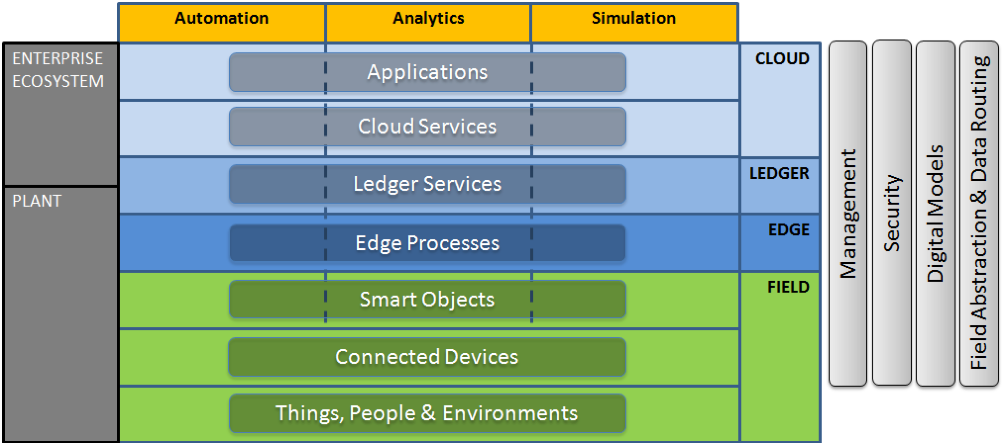
\includegraphics[width=\linewidth]{images/Far-edge.png}
	\caption{FAR-EDGE Reference Architecture overall view}
	\label{fig:architecture}
\end{figure}

As far as simulation is concerned FAR-EDGE aims at providing models and tools entailing functionalities for modeling CPS-based discrete manufacturing factories and simulating their behavior along the whole factory life cycle. 
In the FAR-EDGE vision, in fact, simulation is seen as a first-class citizen of the factory of the future (as it is in I4.0 guidelines), being an enabler to implement layout and product optimization, to test \textit{what-if} scenarios at minimal impact of regular shop activities, or as a the cornerstone to support reactive (\textit{now-what}) operative decisions. 

As was mentioned in the introduction to this chapter, one of the main challenges of simulation in manufacturing is the so-called \textit{Digital Continuity}; it consists in creating the conditions for a model to be up-to-date at any moment during the various phases of the life cycle of a factory. 
Thus, if from one hand this means that the interoperability of the model for virtualization and simulation must be maximized (engineering is by-nature a multidisciplinary process), from the other new mechanisms must be developed and put in place to allow the model to be in-synch with the shop floor evolving as automatically as possible with the state of the factory. As CPSs are subject to changes (e.g., for straining and aging), models should reflect those transformations. To detect this gap and update the model accordingly, raw data from the field (direct) or complex analysis algorithms (from Analytics domain) can be used. However, it is important to point out that the model itself must support model synchronization functionality natively in order to decouple the FAR-EDGE architecture, which must be independent of the particular factory, and the synchronization process that depends on the particular configuration of the factory at hand and ultimately on the model. 
For all the reasons presented above, the task of defining a suitable model is very ambitious; not only FAR-EDGE aims at including in a single harmonic, coherent representation control, communication data collection and simulation data, but also at defining and being able to share a model describing the synchronization process. 

Before being able to present the FAR-EDGE CPS data model and to understand the underlying choices it is important to clarify its relationship with other elements of the reference architecture presented in Figure~\ref{fig:architecture} and in particular with the components related to the simulation domain. 

In Figure~\ref{fig:architectureSimulation} is an excerpt of the overall reference architecture of FAR-EDGE. The simulation domain is envisioned as a layered subsystem of the architecture where the topmost elements are FAR-EDGE-enabled simulation tools and a graphical editor; these rely on the \textit{Open API for Virtualization} to interact with the core of the Simulation subsystem: the CPS Model for Simulation, which is presented in its initial version in this document.

WP4 is responsible for developing and openly providing an API for virtualization that, by means of suitable endpoints allows: 
\begin{itemize}
    \item \textbf{Definition and configuration of simulation scenarios,} including simulation configurations. These will be fully compliant with the FAR-EDGE digital models.
    \item \textbf{Execution of simulation scenarios}, including simulation of CPS systems, machine and devices. FAR-EDGE will support two external simulators in leveraging information and digital models of the inputs and outputs of the CPS systems, along with data mining models and statistics (e.g., time series analysis) that will be used to describe and determine the outputs of the CPS systems during the simulation.
    \item \textbf{Management of digital models synchronization}, including configuration of the Real-to-Digital Synchronization Component and deployment of Synchronization models. 
\end{itemize}


A large number of publications can be found in literature on the topic of simulation; for years, it is considered an established and fundamental tool for the evolution of science. In addition, while with the term simulation we refer to a collection of intuitive concepts, the same is not true for real-to-digital synchronization. For this reason, we dedicate the next section to this topic so that the reader can later easily understand how the data model fulfills the requirement of supporting synchronization.

\begin{figure}
	\centering
	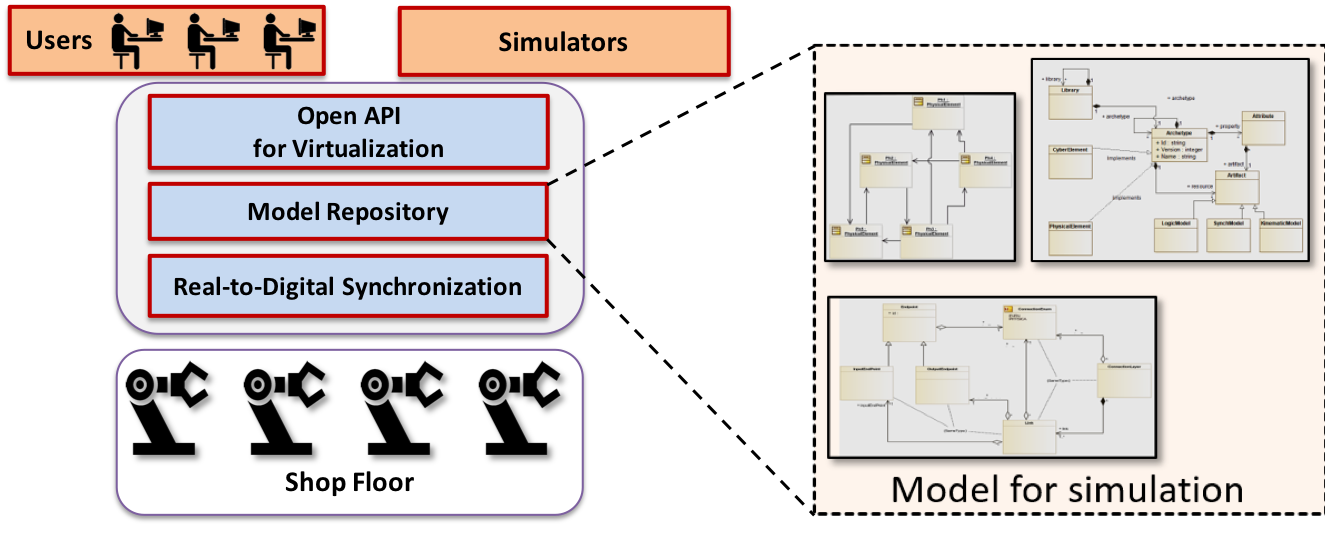
\includegraphics[width=\linewidth]{images/Architecture}
	\caption{Architecture supporting the Digital Continuity}
	\label{fig:architectureSimulation}
\end{figure}



\section{A Model for Simulation and Digital Continuity}\label{sec:model}
The objective of this section is to present the main elements of the CPS simulation and synchronization model. However, in order to understand the underlying choices, it is important to clarify its relationship with other elements of the reference architecture presented in Figure~\ref{fig:architecture} and in particular with the components related to the simulation domain. 

In Figure~\ref{fig:architectureSimulation} is an excerpt of the overall reference architecture of FAR-EDGE. 
The simulation domain is envisioned as a layered subsystem of the architecture where the topmost elements are simulation tools and a graphical editor; these rely on the \textit{Open API for Virtualization} to interact with the \textit{Model Repository}, that manages the CPS-based simulation model, and the \textit{Real-to-Digital Synchronization} module that is in charge of supporting the Digital Continuity. 
In particular, the Model Repository manages the virtual shop floor representation, which relies on a shared modeling of core concepts that can be expanded to suit specific purposes; This, in fact, is required to sustain integration of different domains and provision of cloud-based simulation services. 
Lastly, the simulation domain is responsible for developing and openly providing an API for virtualization that, by means of suitable endpoints allows: 
\begin{itemize}
    \item \textbf{Definition and configuration of simulation scenarios}, that is the platform supports the definition of complete multi-disciplinary CPS models. The API must therefore be able to manipulate the CPS data model to allow the user (or machine constructor) to describe the CPS from different points of view, in order to enable different types of simulations. In addition, the API must support the composition of the CPSs and the subsequent model maintenance.  
    \item \textbf{Execution of simulation scenarios}, including simulation of CPS systems, machine and devices. The platform supports external simulators in leveraging information and digital models of the inputs and outputs of the CPS systems, along with data mining models and statistics (e.g., time series analysis) that are used to describe and determine the outputs of the CPS systems during the simulation.
    \item \textbf{Management of the digital continuity}, that is the process of continuously updating the digital models, including configuration of the Real-to-Digital Synchronization Component and deployment of Synchronization models. 
\end{itemize}



\begin{figure}
	\centering
	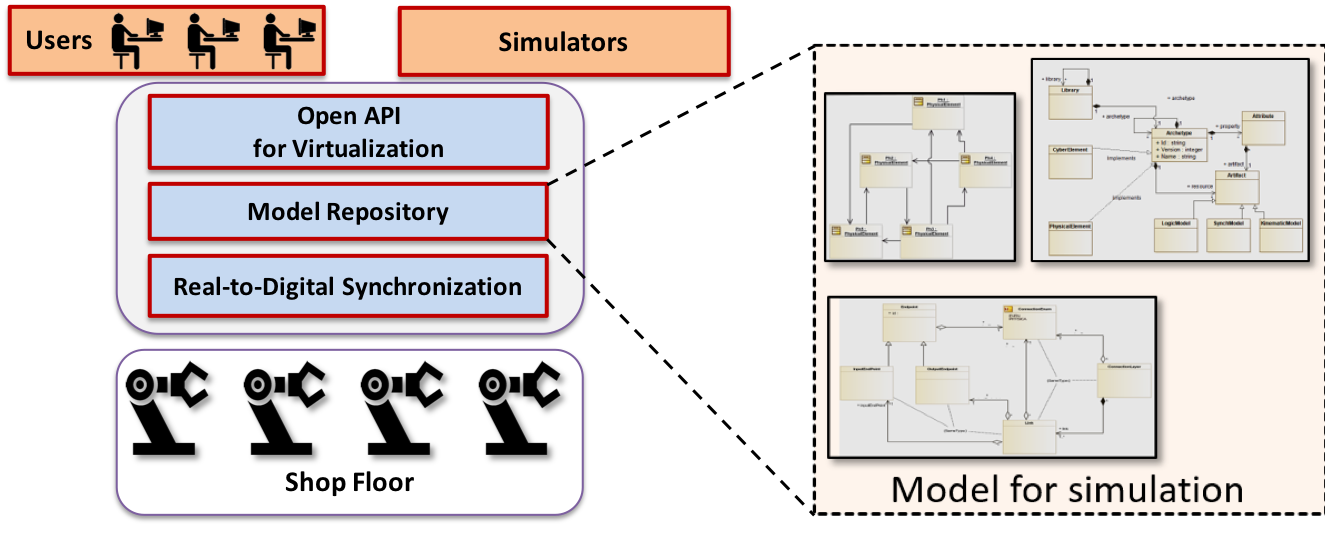
\includegraphics[width=\linewidth]{images/Architecture}
	\caption{Architecture supporting the Digital Continuity}
	\label{fig:architectureSimulation}
\end{figure}





Supporting such ambitious objectives is translated into a set of requirements that data models have to fulfill. 
To this end, our data model needs to be:
\begin{description}
\item[Expressive]- to enable the description of possibly any resource or flow involved in production, logistics and management processes of different industrial domains.
\item[Extensible]- to build, upon a core representation of the factory environment, a growing model ecosystem capable to maintain the digital information available all along the factory life-cycle.
\item[Interoperable]- to provide users with a personalized view and simulation tools that present the virtual environment from their perspective supporting the decision-making processes, activity planning and operation controlling.
\item[Scalable]- that is the ability to function efficiently when the context is changed in size or volume featuring multi-level access features and suitable aggregation patterns.
\item[Modular]- so that it provides representation building blocks that can be rearranged and reconfigured to follow the continuous evolution  of the real factory.
\end{description}


One of the most common features of manufacturing plant design is is to use standardized components (machine tools, robots, etc.) composed in a modular way. 
Through a good organization of modules, in fact, it is possible to speed up engineering as well as the simulation setups, maximizing the reuse of components. 
Similarly, simulation software solutions often provides libraries of models that can be aggregated and extended to assemble full plant layouts.
In this work we aspire to provide the same efficient re-use approach implementing classes to describe resources, called \textit{Archetypes} and \textit{Elements}. %which are instances of such elements and the components of the plant model. 
The Archetype-Element relationship is similar to the one that exists in Object Oriented Programming (OOP)~\cite{wolfgang1994design} between a Class and an Instance (Object) of that class.

Another important requirements is that the resulting data model shall support semantically meaningful collection of relations (referred to as \textit{Layers}). 
We deem particularly important to provide the modelers with a tool to gather links of the same type. 
The idea is to simplify the modeling process by dividing the overall model in several levels. 
By way of example, a first layer may contain the definition of the plant topology with its hierarchies of production resources; the other are graphs that can be used to express relations between resources. 
Logical, electrical, and pneumatic layers are just a few examples of layers.
Finally, in order to achieve flexibility and interoperability the model implements the concept of \textit{artifact}, that is the proposed model support the storage and linking of generic files in the description of the digital twins. 
As a consequence, the modeler can decide to define digital twins using exclusively the syntax and constructs provided by the model (white-box approach), or else use specific and opaque formats whenever (s)he deems it necessary (black-box approach).  
Figure~\ref{fig:layers} illustrates graphically this multi-layer modeling approach. 

\begin{figure}
	\vspace*{-0.5cm}
	\centering
	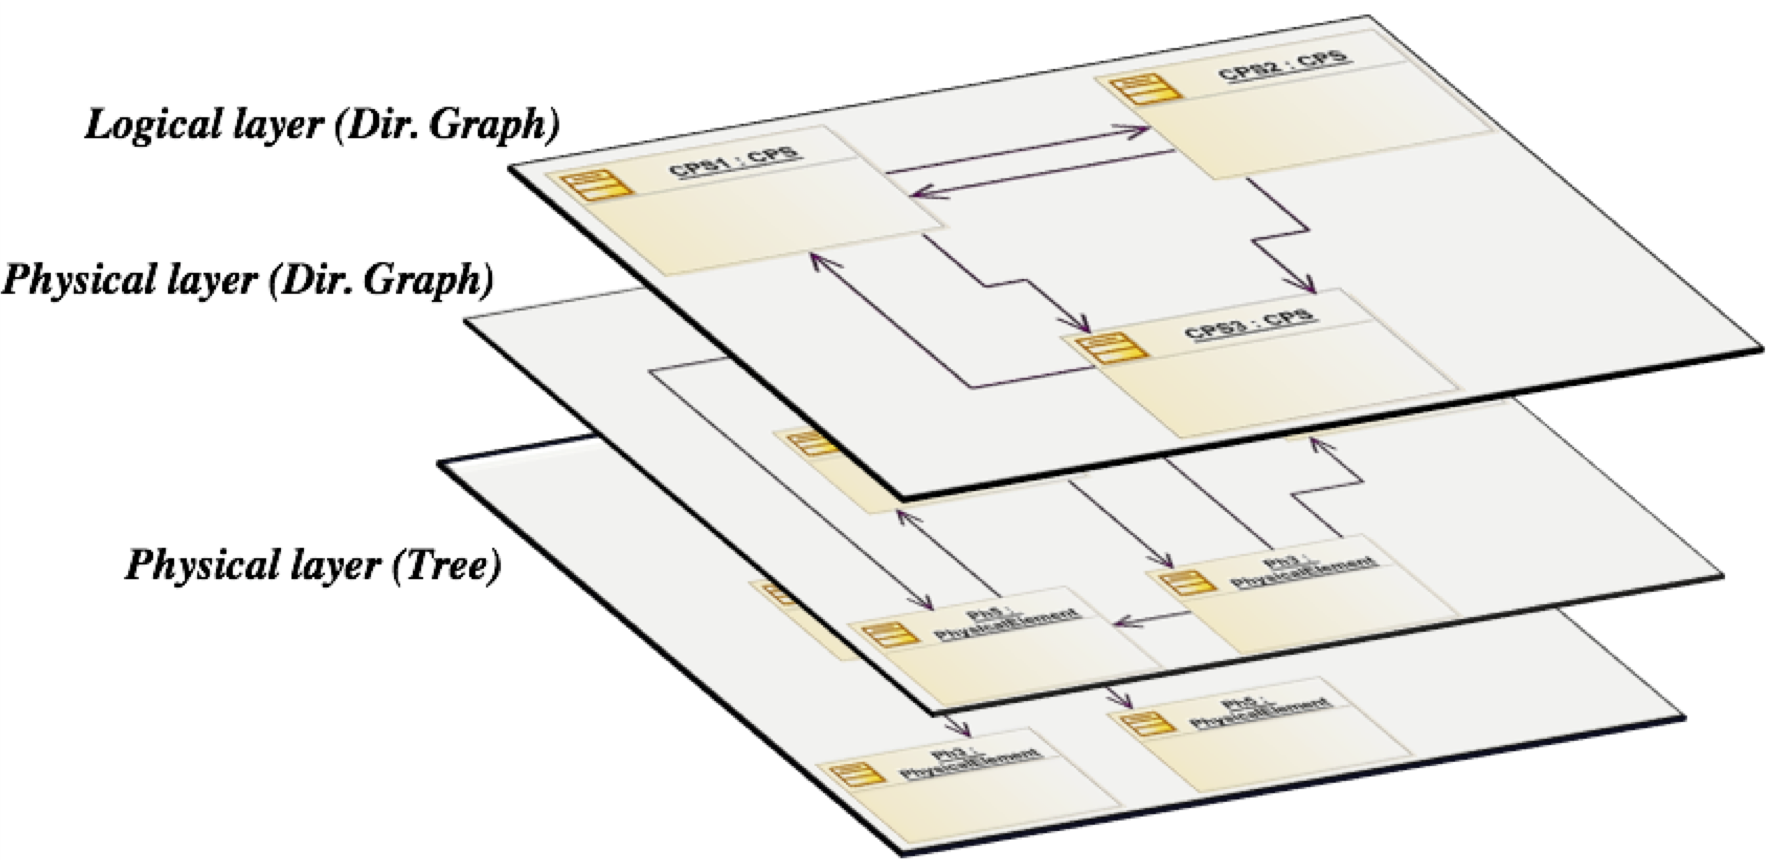
\includegraphics[width=\linewidth]{images/layers2}
	\caption{Modeling using superimposed layers}
	\label{fig:layers}
\end{figure}

This remainder of section documents shortly the data model for simulation and digital continuity, which is organized into 9 areas:

\begin{description}
	\item[\textbf{Core Model}] - documents the core classes used for the definition of  entities and relations used in other sections. The central components of the model are: the \textit{Archetype} and the \textit{Element}. These have a symmetrical structure: both are characterized by one or more roles that identify them semantically, by a unique identifier within the model, by \textit{attributes} (properties used by the modeler to specify Archetypes and Elements), \textit{endpoints} (semantically defined extremes of links connecting Archetypes or Elements) and \textit{artifacts}. 
    \item [\textbf{Archetype Model}] - introduces the concepts of Archetypes as the basis of the model reuse paradigm. Following the OOP paradigm, an Archetype can be seen a moulder that can be used to instantiate \textit{Elements}. The model leaves the user to extend the Archetype concept at will, however, three extensions are provided out-of-the-box, namely, \textit{PhysicalArchetype} (to represent physical resources within a plant), \textit{LogicalArchetype} (to represent the cyber nature of the CPS, used for simulation purposes), and \textit{ProductArchetype} (to represent the semi-finished and the final products of the shop).
	\item[\textbf{Element Model}] - this model presents the concept of Element as instantiation of an Archetype according to the OOP.  As said, Archetypes can be defined as molders used to create specific instances of a certain plant resource. The instances are called Elements. Therefore, Elements are generally created mirroring the structure of their base archetypes, however, unlike  OOP  this is  not  strictly  necessary.  This  means  that  an  element  can  be also defined  as  a  stand-alone  component  or  that  it  is  possible  to add or modify the characteristics inherited from an archetype. 
	\item[\textbf{Connection Model}] - the connection model is devoted to the definition of the links between two model entities.  
To this end, the \textit{Endpoint} class is extended and the concepts of \textit{Link} and \textit{ConnectionLayer} are introduced. 
A Link joins together two instances of the Endpoint class and represents a connection between the elements to which the endpoints belong. 
Links are aggregated in ConnectionLayers and both links and layers can be semantically annotated.

\item[\textbf{Layer Model}] -  extends the concept of layer as a collection of items that can be further specified using attributes. In particular, the user can define collections for Plants (\textit{PlantLayer}), ProductElements (\textit{ProductLayer}), PhysicalElements (\textit{PhysicalLayer}), and LogicalElements (\textit{LogicalLayer}).
	\item[\textbf{Attribute Model}] - specifies the concept of property to be used to annotate other elements of the model, namely Library, Archetype, Artifact, and Endpoint. The concept of attribute is further specified as, among the others, \textit{URI}, \textit{Date}, \textit{Number}, \textit{String}, \textit{Composite}, and \textit{Frame}.
	\item[\textbf{Role Model}] - presents a set of classes that defined the concept of Role as semantic description to further specify the constituent elements of the model. The model allows the user to specify an Element/Archetype by assigning a role to it. The \textit{SemanticRole} is the main class of this model. A role has a unique identifier and a name; furthermore, it can contain attributes and be assigned to a library. Finally, a role can refer to other roles to build tree-shaped semantic relationships and to a parent role in order to support the attribute inheritance.
     	\item[\textbf{Plant Model}] - introduces the Plant as an aggregation of layers representing among other aspects its physical and logical nature.  The \textit{Plant} is the main element of this model; it is a specification of the Element class featuring set of resources (physical, logical, and product) as well as their connections. 
Furthermore, a plant also includes several layers. 
Some of them are mandatory and specific as the physical, logical and product layers, which model hierarchies of physical, logical and product entities, respectively.  Other are optional like one or more generic layers, which model graph-shaped relations among the elements of the mandatory layers. Furthermore, Endpoints can be defined to model connections among plants (via Endpoints).
	\item[\textbf{Project Model}] - documents all the classes that represent multi-plant simulation projects, and enable simulation tools to share plant models, scenarios and results.  
\end{description}

This chapter only reports shortly the main elements of the model due to space limitation; a complete and detailed description of the model can be found in~\cite{Ciavotta2018} and \cite{FAR-EDGE41}.



%\section{Literature Review}
%(\textbf{Andrea})
%brief literature review sistemi plug-and-simulate


\section{Real-to-Digital Synchronization System}
The main requirement of the FAR-EDGE CPS Data Model is to provide full support to the \textit{Open API for Virtualization}. 
In othe words, the data model has to be designed with the goal of : 
\begin{enumerate}
\item providing tools to fully describe simulation models to be imported and executed in one of the two simulators that FAR-EDGE supports
\item allowing the user to define complex synchronization processes to be carried out by the Real-to-Digital Synchronization (R2DS) Component and the \textit{Edge Analytics Engine}. 
\end{enumerate}

The Real-to-Digital Synchronization (R2DS) can be defined as the process of continuously updating CPS models stored in the \textit{Model Repository}, following the evolution of the shop floor. 
Having up-to-date models is especially important in simulation. 
In fact, machines along their life cycle are subject to aging, straining, and reconfiguration processes, which might affect their behavior and performance; in this case the simulation outcomes to drift apart substantially from reality and, therefore, result useless. 
In order to be able to make informed decisions based on reliable simulation models, it is of paramount importance to detect changes in the model automatically and continuously, and to adapt parameters and scenarios accordingly. 

The core of the R2DS grounds in the processing of data gathered at shop floor level. 
It is worth noticing that this is a general approach, based on data processing, which enables not only the tracking of CPS models parameters but it also unlocks scenarios where, for instance, digital twins can be enriched with inferred pieces of information that cannot be directly measured from the field. 
For illustration purposes, let's imagine the case in which a digital twin is extended with the results of a machine learning algorithm for predictive maintenance~\cite{daily2017predictive}. This information, in turn, could be used from the simulation to schedule the most suitable time to perform the maintenance of the real machine.  
Having based the synchronization process on a general-purpose data analytics engine has the non-secondary benefit to leave the overall architecture independent from the simulation domain. The other side of the coin is that, with this approach, the definition of the synchronization procedure must be implemented as part of the data model. 
This is because each digital twin might require a different data processing (a.k.a. \textit{Synchronization Model} - SM) to be synchronized with its real counterpart. 

Synchronization Models describe the way data from the field must be processed to update the model attributes or to estimate indirect values and create new attributes. 
A synchronization model contains an algorithmic description of how to process data from machine sensors at shop floor level in order to generate updates that continuously serve to keep the digital twin digital in sync with the related CPS. 
This description can therefore be instantiated in different ways depending on the technological choices that underlie the implementation of the platform. 
The solution adopted in the project is to implement the synchronization model in the form of a simulation asset, that is a binary file containing executable code and to associate it with the representation of a CPS within the data model. The synchronization model, therefore, in order to perform its duty, must be compiled, installed and managed within a suitable execution environment, which can provide through an API the abstractions necessary to process data coming from the production environment in a distributed way.  


Specific components will be in charge of managing the life cycle of Synchronization Models, which includes: 
\begin{itemize}
\item \textbf{checking the execution schedule}: depending on the synchronization scenario the SM can be continuously executed against streams of field data (if the CPS is reachable and producing data), or it is scheduled to run periodically, say for instance, once a day over historical data. 
\item \textbf{model fetching}: the SM persisted in a suitable database is looked up and retrieved. 
\item \textbf{execution}: the SM is run exploiting FAR-EDGE Open API for Analytics and Synchronization Services
\item \textbf{application of the updates}: the SM generates attribute values for the related digital twin. These values are used to update the digital twin, which the model refers to.
\item \textbf{model dismissal}: once the dismissal condition is verified as, for instance, the CPS is not connected or the synchronization process ended the SM is dismissed and the \textit{Synchronization Services} sub-system is notified.
\end{itemize}

Figure~\ref{fig:r2ds} describes graphically a reference scenario where a CPS, registered and connected to the FAR-EDGE platform, is switched on and a data flow is spawned via the \textit{Data Routing and Preprocessing Component} of the architecture. 
The R2DS Component is notified and, if a SM is associated with the CPS digital twin in the model repository, it will be retrieved and executed on the Synchronization Services, which in turn rely on the Edge Analytics Engine. 
In this scenario, the SM will process the input data flow and generate in output a new one, containing for each time interval the updates to be applied to the corresponding digital twin. 
The R2DS component is in charge of performing the model update process. 
It is worth restating at this point that the algorithm implemented within a SM it is not constrained to the generation of attribute updates for digital twins, but it is general. In this way, for instance, the same infrastructure and the overall process can be used to enrich the CPS definition with new pieces of information. 

\begin{figure}
	\centering
	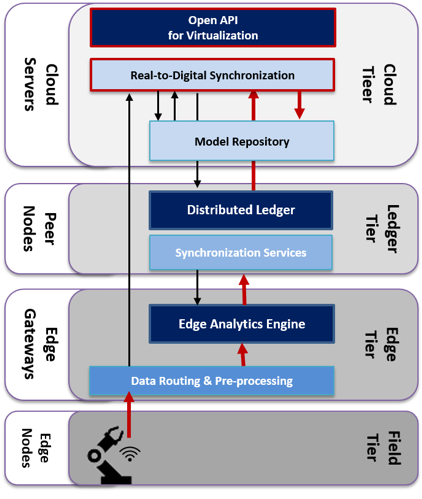
\includegraphics[width=0.6\linewidth]{images/R2DS}
	\caption{Synchronization process in the scenario of data stream processing}
	\label{fig:r2ds}
\end{figure}




\subsection{The Architecture}\label{sec:architecture}
%Accurate simulations of all stages of the production process is of crucial importance to make decisions aimed to speed up the performance improvement of a shop floor. 
%Applying discrete simulation techniques to a traditional shop floor can be a resource and time consuming process mainly due to data inaccuracies as even small variations of production parameters might lead to divergent simulation results compared to the actual system.

%In the industry 4.0 context, the shop floor is made by self-monitoring production machines and robots, namely CPS, with the capability to share their own state information with other stakeholders. Through a connection layer, this information can be exchanged and stored and used for achieving more realistic simulation input data which, in turn, leads to more accurate forecasting capabilities. In this way, the factory behavior can be accurately predicted in advance. Moreover, thanks to this quasi real-time mirroring of real elements into their virtual representation, it is possible to simulate on current data thus exploiting simulation potentials not only in the factory design and planning phase but also in the operative one. This allows to perform what-if analysis on the current production situation in order to support decision-making processes aimed at improving performances typically outside the boundaries of simulation such as ensuing the on-time delivery of customer orders or reallocating production resources to balance the current production.


In the FAR-EDGE Architecture (Figure~\ref{fig:r2ds}) several technological tiers are foreseen (from Field to Cloud) and the \textit{Real-to-Digital Synchronization} component is located in the uppermost tier, the Cloud Tier. Nevertheless, this component must also work closely with the other elements of the architecture to fulfill its role. Schematically (and referring only to the process of updating the digital twins stored in the \textit{Model Repository}), the Real-to-Digital Synchronization component must be able to access the services offered by the Edge layer and this is accomplished by means of the use of a system data bus. 

\begin{figure}[t]
  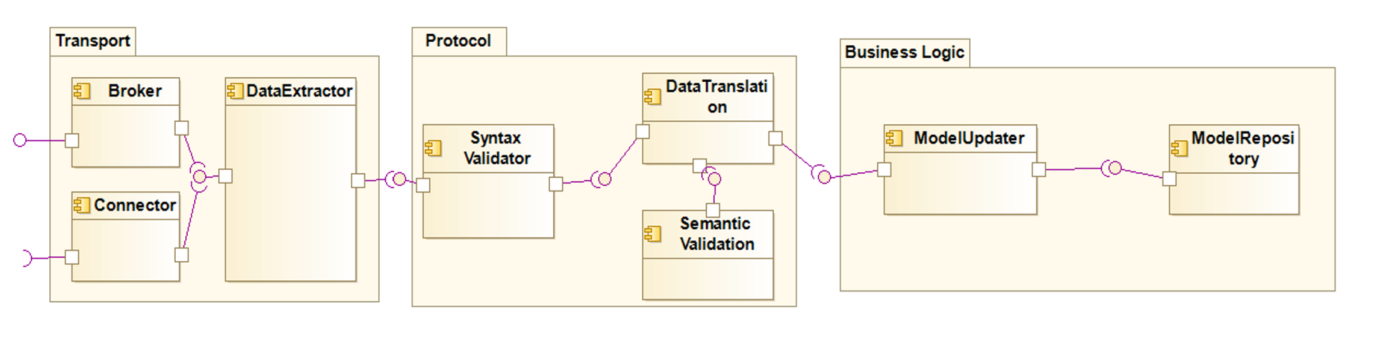
\includegraphics[width=\linewidth]{images/diagramComponent.PNG}
  \caption{Real to Digital Synchronization Component Diagram}
  \label{fig:realToDigitalComponentDia}
\end{figure}

Figure~\ref{fig:realToDigitalComponentDia} details the internal elements of the Real to Digital Synchronization component. 
Three main units interact to carry out the synchronization process, namely:
\begin{description}
\item The \textbf{Data Client}, which is the component in charge of bridging the physical to the digital world. Specifically, the main objective of this component is to provide access to the data produced in the Field tier. This is achieved in two ways:
\begin{enumerate}
\item The first way is to access the data through a registered broker in a \textit{PUSH} mode, meaning that the client is notified if new data is available.
\item The second way is to send a request using a client named in Figure~\ref{fig:realToDigitalComponentDia} as \textbf{Connector} in a \textit{PULL} mode, meaning that the client is responsible for asking if new data is available. An example of Connector can be a HTTP Client.
\end{enumerate}
Both the data connection modes communicate with the \textbf{Data Extractor} component, which is responsible for eliciting the information sent through the communication channel. 
The output of this component is a pure SenML~\cite{jennings2018sensor} data structure. SenML is a specification to define sensor measurement and it provide the possibility of being represented by different formats including XML and JSON. The SenML excerpt in Figure~\ref{fig:senML} represents the sensor reading of an item that has just been produced and informs the transport process to store the it in the warehouse. In addition to the name of the sensor and the timestamp of the measurement, in the message, other information are provided such as the serial number and the production line where the product has been assembled.

\begin{figure}[h]
  \frame{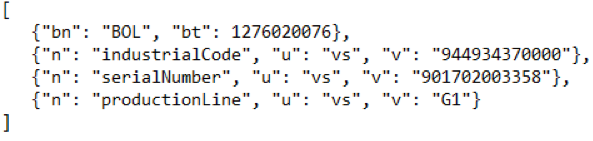
\includegraphics[width=0.7\linewidth]{images/senMl.png}}
  \caption{Example of message in SenML format}
  \label{fig:senML}
\end{figure}

The main advantage of this approach is that the underlying technologies responsible for communicating the message can be decoupled from the content of the message itself. 
By replacing the particular broker or connector, indeed, the component can be adapted to any communication protocol. 
%A prototype of this component is available in the Test Environment that is presented in Section \textbf{XXXX} In that version, the Data Client uses a subscription to a Kafka Channel that provides the functionalities of Broker and \textit{DataExtractor}.

\item The \textbf{Format Manager}, which is responsible for managing the data format. Since in the project vision each CPS vendor will be responsible for defining the message format, both semantically and syntactically, a specific component able to deal with conversion issues is required.
This component receives from the \textit{Data Client} a message containing the incoming serialized information from the shop floor. 
This message undergoes a first syntax check using a specific JSON-schema performed by the \textbf{Syntax Validator}. 
Afterwards, the whole message is parsed by the \textbf{Data Translator}, where a second check about the semantics is performed. 
Finally, the information is translated into an internal format required by the next component of the architecture. 

\item The \textbf{Business Logics Manager}, which is responsible for organizing the data in the Simulation \textit{Model Repository}. The main responsibility of this component is to map the data contained in the sensor message with the specific data model instantiated in the model repository component.
After the message parsing phase, the shop floor data is validated and is available for the comparison with the corresponding model repository data.
\end{description}



The remainder of this section details the interactions among the aforementioned. In the sequence diagrams shown in Figure~\ref{fig:r2dssequence} the overall real to digital synchronization workflow is presented.
The initial step in order to align the platform with the available sensor data is to connect it to the shop floor. 
The platform receives from the Monitoring App, through a \textit{PlatformCommandHandler} the \textit{ConnectPlatform} message. 
This causes a request to the \textit{FaredgeAPI} (that abstracts the interface with the architecture) which returns the list of active CPS.
For each CPS that is found, its specific configuration is loaded. The configuration specify if a synchronization model is associated with the particular CPS.  In case of a positive response, the platform instantiates a synchronization component, connects it to the CPS data sources and executes the model. Thereinafter all the active CPS are subscribed to the data bus topic, and can send their own sensor data.


\begin{sidewaysfigure}
  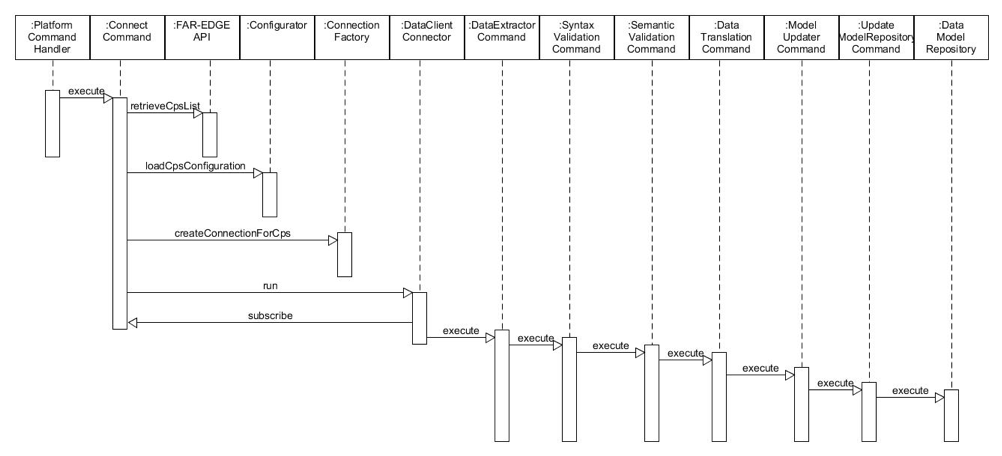
\includegraphics[width=\textheight]{images/R2DSsequence.png}
  \caption{Real-to-Digital Synchronization process - Sequence Diagram}
  \label{fig:r2dssequence}
\end{sidewaysfigure}


When a CPS communicates new sensor data, the \textit{DataClientConnector} is invoked. Its main responsibility is to activate the \textit{DataExtractor}; this reads the topic and the sensor data from the communication channel and forwards them to the \textit{SyntaxValidator}.
During this step the message is verified using the appropriate JSON schema. If the data format is recognized, a second validation is made. In this phase the values are checked in order to ensure the semantic quality of the data.
Upon successful completion of the second validation, the sensor data are sent to the \textit{DataTranslator}. This component provides a translation into a common internal format. After this step the message is totally decoupled from its original format. That allows to use different data formats, potentially one for each CPS. 


The virtualization and simulation platform has been developed and tested in a laboratory environment with particular reference to the case study presented in the next section. Notably, in addition to the components just described, a web application for graphical monitoring has been created that allows the user to manage the system remotely. Figure~\ref{fig:wizard} shows a screenshot of this application. 
In order to allow any vendor to create their own implementations of real to digital, a graphical interface has been developed in the project. 
By means of a wizard, this graphical interface allows the user to manage the behaviour of that component. 
Three main functionalities are exposed
\begin{description}


\item \textit{Download Archetype}: In this step, the person responsible for the real-to-digital of a CPS can download a Archetype containing the framework classes needed to implement the CPS digital twin and the synchronization process. The package also contains the parsing libraries to streamline the developing and testing processes.
\item \textit{Upload}: Once the component development is complete, the user can upload the CPS digital twin to the platform.
\item \textit{Pairing}: This interface shows the list of CPS currently connected to the platform along with their synchronization models (if available). The user can manually pair the CPS with the model. It is possible to associate a different model to each CPS or reuse an existing one according to the use case.
\item \textit{Activation}: At this point the CPSs connected to the platform are associated with the real to digital drivers. As the last step is just to activate the CPS so as to allow the connection and start receiving the synchronization of data. The CPS can be deactivated at any time in order to allow, for example, updates to the synchronization models.
\end{description}

\begin{figure}
  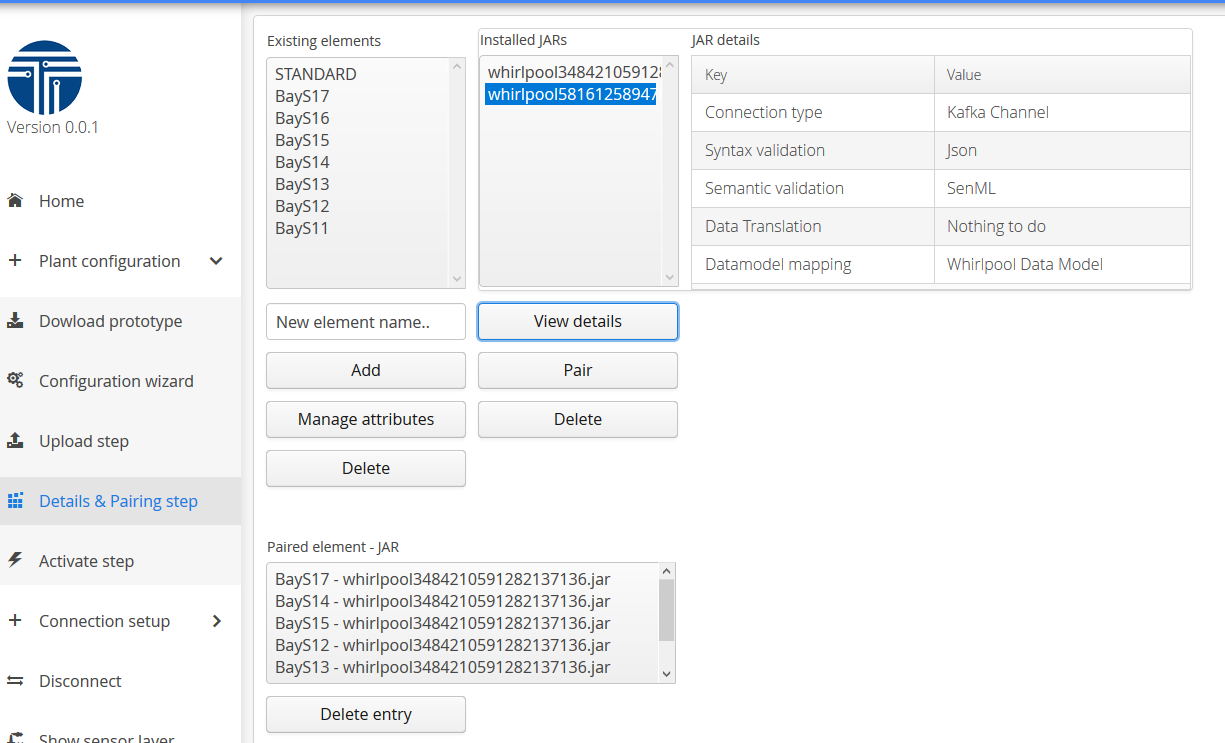
\includegraphics[width=\linewidth]{images/wizard.PNG}
  \caption{Real to Digital Synchronization wizard}
  \label{fig:wizard}
\end{figure}









\section{Case Study}\label{sec:caseStudy}
(Ha cominciato michele, per favore riguardare ed estendere \textbf{Andrea} \textbf{Gabriele}
The rationale of this section is to present the use case scenario (the one we call hereinafter Melano Sorter) that will be used throughout the document as the roadway lines to explain concepts and adopted solutions.
The use case describes the hob handling and palletizing operations carried out by within the Melano production plant in Italy (Whirlpool). The elements characterizing this use case scenario from the simulation viewpoint are reported below:

\begin{itemize}
\item In the plant situated in Melano Whirlpool produces over a hundred different configurations of cooking hobs, belonging to three categories: gas, electric or pyro-ceramic. The production is organized in batches;  hobs the same type are aggregated taking into account different orders. Each batch (and every hob in it)  is identified by a code to ensure a high level of traceability. For the same reason, as soon as a single hob is released, an automated reading system records its associated event and communicates it in real-time to the ERP. 
\item The cooking hobs are realized by 14 production stations; each station produces one hob at a time and it is specialized in producing items of only one category (gas, electric, pyro-ceramic).  The automation of the production lines is achieved by means PLCs connected to a MES. Seven palletizers are placed at the end of the stations; they have the task of aggregating in a pallet (generally) 6 elements belonging to the same lot and assigning a unique 2D barcode to the pallet. Small differences in lot size are to be ascribed to the quality control process (affecting about 2\% of items produced). The pallets are then taken over by a raised conveyor of about 1 kilometer long. The length of the conveyor, its average speed as well as the shelf life of the pallets on it are known data of the problem. 
\item On the end of the conveyor there is a 2D barcode reader and a PLC-based automation system, which we refer to hereinafter with the term "Sorter". The sorter has the task of assigning the pallets out of the conveyor to different shipping lines. The barcode reader is placed between the end of the conveyor and the sorter. In this way the sorter becomes aware of the particular type of product contained in the pallet and can decide on which output line (also referred to as “Bay”) to allocate it. The sorter, at the beginning of the earliest shift, assigning each available bay to a particular type of hob. Moreover, depending on the particular production plan, a particular hob type can be assigned to more than one bay. Please notice that, until the next day the hob type/shipping line configuration cannot be modified. 
\item The Melano Whirlpool plant features 18 shipping lines (bays) freely assignable to any type of product. There is also a further bay, which will be indicated by the phrase "mixed bay" to which the sorter directs all those pallets that can not be assigned to regular bays. Finally, there is a bay for incomplete pallets. Regular bays are handled through a forklift that picks up pallets and places them in the corresponding area of the warehouse, whereas the  mixed and incomplete bays pallets are handled manually.
\end{itemize}
	
Figure~\ref{fig:sorter1} below shows schematically the "Sorter" sub-system of the Melano plant.
In the vision of the FAR-EDGE project, Whirlpool will benefit from modeling and simulation of this use case as it will be possible to evaluate different layout configurations and operating logics for the "sorter" without actually stopping the production and implementing the changes. Therefore, working in partnership with WP6, we will act in two successive phases:
\begin{itemize}
\item In the first phase we will create a simulation model (to be run in a Discrete Events Simulator – DES) capable of faithfully representing the current configuration of Melano site. To do this we will analyze the data that Whirlpool will make available to the consortium; to assess the suitability of the model to represent the status quo, we will compare the KPI values obtained through simulation with those measured in the field. This work will be done mainly within the WP4.
\item In the second phase, a what-if analysis will be carried out using alternative simulation scenarios in which the layout (for example, the number of shipping bays) or the algorithm implemented within the "sorter" will be changed. The goal of this phase is to identify margins of improvement with respect to the current situation. This second phase will focus on WP6. Example of questions to be answered in the what-if analysis are:
\begin{itemize}
\item In case of a capacity increase, will the sorter able to manage the normal flow?
\item In case of production plan changes; will the sorter able to manage the normal flow? 
\item In case of production mix changes; will the sorter able to manage the normal flow? 
\item In case of physical reconfigurations, will the sorter able to manage the normal flow? 
\end{itemize}
\end{itemize}


As for T4.1, and specifically this document, this use case scenario has been select among the others for its simplicity; therefore, it can be easily used to explain the various elements of the FAR-EDGE CPS data model and the transformation rules from our from internal model to other formats like JSON.

\begin{figure}
	\centering
	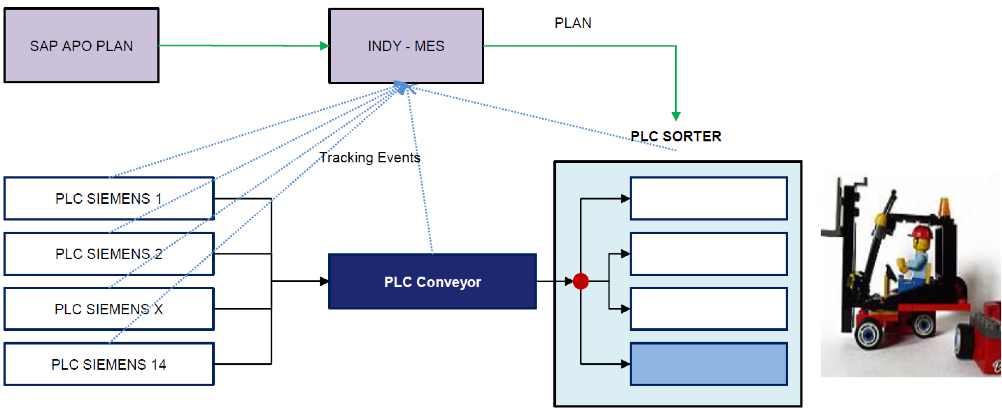
\includegraphics[width=\linewidth]{images/Melano1}
	\caption{Melano sorter use case scenario}
	\label{fig:sorter1}
\end{figure}



\section{The vision: digital-to-real}
This Section collects a number of considerations accrued in the frame of this research about the future (if not immediate at least near) of simulation applied to industrial environments. 
We refer with the phrase \textit{simulation-in-the-loop}, the set of processes that realize the virtual factory (real-to-digital) and those that enable the application of the results of the simulation to the real factory (digital-to-real). 
In fact, since the objective of this Chapter is to document the feasibility of a platform capable of managing digital twins so that they faithfully and continuously reflect the state of their real counterpart, it has been intentionally left little room for the downstream decision-making process of the simulation. 
This is because at the moment, in many contexts, it can be still cumbersome to operate on the real system to implement the insights obtained through simulation. 
Nevertheless, at least in two scenarios it is possible to imagine to close the loop and act directly on the processes of the real factory. 

The first scenario concerns the reaction to unexpected events, such as the arrival of a particularly important order or a machine breakdown; in cases like these the simulation can be very useful to react swiftly by generating alternative configurations. Since the production is already managed digitally by means of MES/ERP software applications, we can imagine a full integration between the mechanisms of planning and management of the production and the simulation to achieve a flexible and reactive manufacturing. 

In the second scenario we can imagine to interact with the cyber nature of a CPS. The relationship between software run by CPS and simulation tools is already very close. The simulated reality allows in fact to test the behavior of a machine before actually placing it in a production line. This approach has the advantage of shortening development times and improving factory safety. Once production has started, however, during the CPS life cycle it may be necessary to update the software for various reasons. Therefore, one can picture a system that, being able to take advantage of the constantly updated digital twin, can automatically adjust the settings of the software in order to make it always work in optimal conditions or even improve its performance (speed of operation, power consumption, and so on). The new code can, after being validated by a human expert, be uploaded directly to the CPS reducing to a minimum the downtime of the line. 


\section{Conclusions}
In questa sezione dobbiamo fare un veloce recap di quello che è stato detto nel capitolo, fare riferimento al caso di studio.
Inoltre come lavoro futuro dire che per ora ci siamo limitati ad implementare una piattaforma che è in esecuzione sul cloud. Lasciando all'Edge computing solo la gestione distribuita dei processi di analytics, mentre nel futuro lavoreremo per spostare parte della simulazione sui CPS cercando di risolvere problematiche relative al deployment, all'esecuzione realtime dei processi senza influire negativamente sul lavoro del CPS e quindi sulla produzione. 
%\appendix

%And this is my Appendix.

%\subsection*{Appendix Subsection}

%Some text.

%\nocite{*} % add all entries from sample.bib

\bibliography{chapter.bib}

\end{document}
